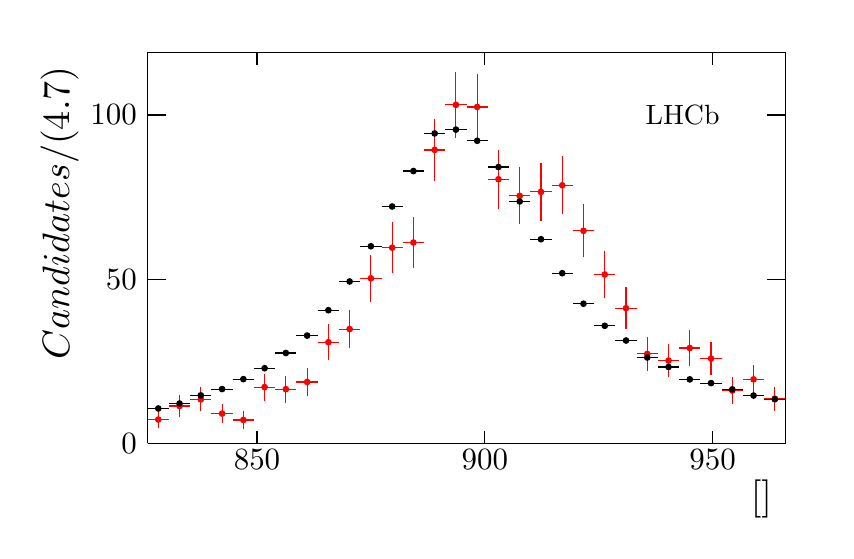
\begin{tikzpicture}
\pgfdeclareplotmark{cross} {
\pgfpathmoveto{\pgfpoint{-0.3\pgfplotmarksize}{\pgfplotmarksize}}
\pgfpathlineto{\pgfpoint{+0.3\pgfplotmarksize}{\pgfplotmarksize}}
\pgfpathlineto{\pgfpoint{+0.3\pgfplotmarksize}{0.3\pgfplotmarksize}}
\pgfpathlineto{\pgfpoint{+1\pgfplotmarksize}{0.3\pgfplotmarksize}}
\pgfpathlineto{\pgfpoint{+1\pgfplotmarksize}{-0.3\pgfplotmarksize}}
\pgfpathlineto{\pgfpoint{+0.3\pgfplotmarksize}{-0.3\pgfplotmarksize}}
\pgfpathlineto{\pgfpoint{+0.3\pgfplotmarksize}{-1.\pgfplotmarksize}}
\pgfpathlineto{\pgfpoint{-0.3\pgfplotmarksize}{-1.\pgfplotmarksize}}
\pgfpathlineto{\pgfpoint{-0.3\pgfplotmarksize}{-0.3\pgfplotmarksize}}
\pgfpathlineto{\pgfpoint{-1.\pgfplotmarksize}{-0.3\pgfplotmarksize}}
\pgfpathlineto{\pgfpoint{-1.\pgfplotmarksize}{0.3\pgfplotmarksize}}
\pgfpathlineto{\pgfpoint{-0.3\pgfplotmarksize}{0.3\pgfplotmarksize}}
\pgfpathclose
\pgfusepathqstroke
}
\pgfdeclareplotmark{cross*} {
\pgfpathmoveto{\pgfpoint{-0.3\pgfplotmarksize}{\pgfplotmarksize}}
\pgfpathlineto{\pgfpoint{+0.3\pgfplotmarksize}{\pgfplotmarksize}}
\pgfpathlineto{\pgfpoint{+0.3\pgfplotmarksize}{0.3\pgfplotmarksize}}
\pgfpathlineto{\pgfpoint{+1\pgfplotmarksize}{0.3\pgfplotmarksize}}
\pgfpathlineto{\pgfpoint{+1\pgfplotmarksize}{-0.3\pgfplotmarksize}}
\pgfpathlineto{\pgfpoint{+0.3\pgfplotmarksize}{-0.3\pgfplotmarksize}}
\pgfpathlineto{\pgfpoint{+0.3\pgfplotmarksize}{-1.\pgfplotmarksize}}
\pgfpathlineto{\pgfpoint{-0.3\pgfplotmarksize}{-1.\pgfplotmarksize}}
\pgfpathlineto{\pgfpoint{-0.3\pgfplotmarksize}{-0.3\pgfplotmarksize}}
\pgfpathlineto{\pgfpoint{-1.\pgfplotmarksize}{-0.3\pgfplotmarksize}}
\pgfpathlineto{\pgfpoint{-1.\pgfplotmarksize}{0.3\pgfplotmarksize}}
\pgfpathlineto{\pgfpoint{-0.3\pgfplotmarksize}{0.3\pgfplotmarksize}}
\pgfpathclose
\pgfusepathqfillstroke
}
\pgfdeclareplotmark{newstar} {
\pgfpathmoveto{\pgfqpoint{0pt}{\pgfplotmarksize}}
\pgfpathlineto{\pgfqpointpolar{44}{0.5\pgfplotmarksize}}
\pgfpathlineto{\pgfqpointpolar{18}{\pgfplotmarksize}}
\pgfpathlineto{\pgfqpointpolar{-20}{0.5\pgfplotmarksize}}
\pgfpathlineto{\pgfqpointpolar{-54}{\pgfplotmarksize}}
\pgfpathlineto{\pgfqpointpolar{-90}{0.5\pgfplotmarksize}}
\pgfpathlineto{\pgfqpointpolar{234}{\pgfplotmarksize}}
\pgfpathlineto{\pgfqpointpolar{198}{0.5\pgfplotmarksize}}
\pgfpathlineto{\pgfqpointpolar{162}{\pgfplotmarksize}}
\pgfpathlineto{\pgfqpointpolar{134}{0.5\pgfplotmarksize}}
\pgfpathclose
\pgfusepathqstroke
}
\pgfdeclareplotmark{newstar*} {
\pgfpathmoveto{\pgfqpoint{0pt}{\pgfplotmarksize}}
\pgfpathlineto{\pgfqpointpolar{44}{0.5\pgfplotmarksize}}
\pgfpathlineto{\pgfqpointpolar{18}{\pgfplotmarksize}}
\pgfpathlineto{\pgfqpointpolar{-20}{0.5\pgfplotmarksize}}
\pgfpathlineto{\pgfqpointpolar{-54}{\pgfplotmarksize}}
\pgfpathlineto{\pgfqpointpolar{-90}{0.5\pgfplotmarksize}}
\pgfpathlineto{\pgfqpointpolar{234}{\pgfplotmarksize}}
\pgfpathlineto{\pgfqpointpolar{198}{0.5\pgfplotmarksize}}
\pgfpathlineto{\pgfqpointpolar{162}{\pgfplotmarksize}}
\pgfpathlineto{\pgfqpointpolar{134}{0.5\pgfplotmarksize}}
\pgfpathclose
\pgfusepathqfillstroke
}
\definecolor{c}{rgb}{1,1,1};
\draw [color=c, fill=c] (0,0) rectangle (10,6.27517);
\draw [color=c, fill=c] (1.4,1.00403) rectangle (9.5,5.96141);
\definecolor{c}{rgb}{0,0,0};
\draw [c] (1.4,1.00403) -- (1.4,5.96141) -- (9.5,5.96141) -- (9.5,1.00403) -- (1.4,1.00403);
\definecolor{c}{rgb}{1,1,1};
\draw [color=c, fill=c] (1.4,1.00403) rectangle (9.5,5.96141);
\definecolor{c}{rgb}{0,0,0};
\draw [c] (1.4,1.00403) -- (1.4,5.96141) -- (9.5,5.96141) -- (9.5,1.00403) -- (1.4,1.00403);
\definecolor{c}{rgb}{1,0,0};
\draw [c,line width=0.4] (1.535,1.19341) -- (1.535,1.30552);
\draw [c,line width=0.4] (1.535,1.30552) -- (1.535,1.41763);
\draw [c,line width=0.4] (1.4,1.30552) -- (1.535,1.30552);
\draw [c,line width=0.4] (1.535,1.30552) -- (1.67,1.30552);
\foreach \P in {(1.535,1.30552)}{\draw[mark options={color=c,fill=c},mark size=2.402402pt,mark=*,mark size=1pt] plot coordinates {\P};}
\draw [c,line width=0.4] (1.805,1.33686) -- (1.805,1.47733);
\draw [c,line width=0.4] (1.805,1.47733) -- (1.805,1.6178);
\draw [c,line width=0.4] (1.67,1.47733) -- (1.805,1.47733);
\draw [c,line width=0.4] (1.805,1.47733) -- (1.94,1.47733);
\foreach \P in {(1.805,1.47733)}{\draw[mark options={color=c,fill=c},mark size=2.402402pt,mark=*,mark size=1pt] plot coordinates {\P};}
\draw [c,line width=0.4] (2.075,1.40862) -- (2.075,1.561);
\draw [c,line width=0.4] (2.075,1.561) -- (2.075,1.71338);
\draw [c,line width=0.4] (1.94,1.561) -- (2.075,1.561);
\draw [c,line width=0.4] (2.075,1.561) -- (2.21,1.561);
\foreach \P in {(2.075,1.561)}{\draw[mark options={color=c,fill=c},mark size=2.402402pt,mark=*,mark size=1pt] plot coordinates {\P};}
\draw [c,line width=0.4] (2.345,1.25551) -- (2.345,1.38085);
\draw [c,line width=0.4] (2.345,1.38085) -- (2.345,1.50619);
\draw [c,line width=0.4] (2.21,1.38085) -- (2.345,1.38085);
\draw [c,line width=0.4] (2.345,1.38085) -- (2.48,1.38085);
\foreach \P in {(2.345,1.38085)}{\draw[mark options={color=c,fill=c},mark size=2.402402pt,mark=*,mark size=1pt] plot coordinates {\P};}
\draw [c,line width=0.4] (2.615,1.18906) -- (2.615,1.30018);
\draw [c,line width=0.4] (2.615,1.30018) -- (2.615,1.41129);
\draw [c,line width=0.4] (2.48,1.30018) -- (2.615,1.30018);
\draw [c,line width=0.4] (2.615,1.30018) -- (2.75,1.30018);
\foreach \P in {(2.615,1.30018)}{\draw[mark options={color=c,fill=c},mark size=2.402402pt,mark=*,mark size=1pt] plot coordinates {\P};}
\draw [c,line width=0.4] (2.885,1.54514) -- (2.885,1.71763);
\draw [c,line width=0.4] (2.885,1.71763) -- (2.885,1.89011);
\draw [c,line width=0.4] (2.75,1.71763) -- (2.885,1.71763);
\draw [c,line width=0.4] (2.885,1.71763) -- (3.02,1.71763);
\foreach \P in {(2.885,1.71763)}{\draw[mark options={color=c,fill=c},mark size=2.402402pt,mark=*,mark size=1pt] plot coordinates {\P};}
\draw [c,line width=0.4] (3.155,1.5218) -- (3.155,1.69104);
\draw [c,line width=0.4] (3.155,1.69104) -- (3.155,1.86027);
\draw [c,line width=0.4] (3.02,1.69104) -- (3.155,1.69104);
\draw [c,line width=0.4] (3.155,1.69104) -- (3.29,1.69104);
\foreach \P in {(3.155,1.69104)}{\draw[mark options={color=c,fill=c},mark size=2.402402pt,mark=*,mark size=1pt] plot coordinates {\P};}
\draw [c,line width=0.4] (3.425,1.6022) -- (3.425,1.78233);
\draw [c,line width=0.4] (3.425,1.78233) -- (3.425,1.96247);
\draw [c,line width=0.4] (3.29,1.78233) -- (3.425,1.78233);
\draw [c,line width=0.4] (3.425,1.78233) -- (3.56,1.78233);
\foreach \P in {(3.425,1.78233)}{\draw[mark options={color=c,fill=c},mark size=2.402402pt,mark=*,mark size=1pt] plot coordinates {\P};}
\draw [c,line width=0.4] (3.695,2.05616) -- (3.695,2.28747);
\draw [c,line width=0.4] (3.695,2.28747) -- (3.695,2.51879);
\draw [c,line width=0.4] (3.56,2.28747) -- (3.695,2.28747);
\draw [c,line width=0.4] (3.695,2.28747) -- (3.83,2.28747);
\foreach \P in {(3.695,2.28747)}{\draw[mark options={color=c,fill=c},mark size=2.402402pt,mark=*,mark size=1pt] plot coordinates {\P};}
\draw [c,line width=0.4] (3.965,2.20873) -- (3.965,2.45465);
\draw [c,line width=0.4] (3.965,2.45465) -- (3.965,2.70057);
\draw [c,line width=0.4] (3.83,2.45465) -- (3.965,2.45465);
\draw [c,line width=0.4] (3.965,2.45465) -- (4.1,2.45465);
\foreach \P in {(3.965,2.45465)}{\draw[mark options={color=c,fill=c},mark size=2.402402pt,mark=*,mark size=1pt] plot coordinates {\P};}
\draw [c,line width=0.4] (4.235,2.80384) -- (4.235,3.09941);
\draw [c,line width=0.4] (4.235,3.09941) -- (4.235,3.39497);
\draw [c,line width=0.4] (4.1,3.09941) -- (4.235,3.09941);
\draw [c,line width=0.4] (4.235,3.09941) -- (4.37,3.09941);
\foreach \P in {(4.235,3.09941)}{\draw[mark options={color=c,fill=c},mark size=2.402402pt,mark=*,mark size=1pt] plot coordinates {\P};}
\draw [c,line width=0.4] (4.505,3.16634) -- (4.505,3.48816);
\draw [c,line width=0.4] (4.505,3.48816) -- (4.505,3.80997);
\draw [c,line width=0.4] (4.37,3.48816) -- (4.505,3.48816);
\draw [c,line width=0.4] (4.505,3.48816) -- (4.64,3.48816);
\foreach \P in {(4.505,3.48816)}{\draw[mark options={color=c,fill=c},mark size=2.402402pt,mark=*,mark size=1pt] plot coordinates {\P};}
\draw [c,line width=0.4] (4.775,3.22739) -- (4.775,3.5534);
\draw [c,line width=0.4] (4.775,3.5534) -- (4.775,3.87941);
\draw [c,line width=0.4] (4.64,3.5534) -- (4.775,3.5534);
\draw [c,line width=0.4] (4.775,3.5534) -- (4.91,3.5534);
\foreach \P in {(4.775,3.5534)}{\draw[mark options={color=c,fill=c},mark size=2.402402pt,mark=*,mark size=1pt] plot coordinates {\P};}
\draw [c,line width=0.4] (5.045,4.33517) -- (5.045,4.72926);
\draw [c,line width=0.4] (5.045,4.72926) -- (5.045,5.12335);
\draw [c,line width=0.4] (4.91,4.72926) -- (5.045,4.72926);
\draw [c,line width=0.4] (5.045,4.72926) -- (5.18,4.72926);
\foreach \P in {(5.045,4.72926)}{\draw[mark options={color=c,fill=c},mark size=2.402402pt,mark=*,mark size=1pt] plot coordinates {\P};}
\draw [c,line width=0.4] (5.315,4.87874) -- (5.315,5.30204);
\draw [c,line width=0.4] (5.315,5.30204) -- (5.315,5.72534);
\draw [c,line width=0.4] (5.18,5.30204) -- (5.315,5.30204);
\draw [c,line width=0.4] (5.315,5.30204) -- (5.45,5.30204);
\foreach \P in {(5.315,5.30204)}{\draw[mark options={color=c,fill=c},mark size=2.402402pt,mark=*,mark size=1pt] plot coordinates {\P};}
\draw [c,line width=0.4] (5.585,4.85338) -- (5.585,5.27537);
\draw [c,line width=0.4] (5.585,5.27537) -- (5.585,5.69736);
\draw [c,line width=0.4] (5.45,5.27537) -- (5.585,5.27537);
\draw [c,line width=0.4] (5.585,5.27537) -- (5.72,5.27537);
\foreach \P in {(5.585,5.27537)}{\draw[mark options={color=c,fill=c},mark size=2.402402pt,mark=*,mark size=1pt] plot coordinates {\P};}
\draw [c,line width=0.4] (5.855,3.98341) -- (5.855,4.35731);
\draw [c,line width=0.4] (5.855,4.35731) -- (5.855,4.7312);
\draw [c,line width=0.4] (5.72,4.35731) -- (5.855,4.35731);
\draw [c,line width=0.4] (5.855,4.35731) -- (5.99,4.35731);
\foreach \P in {(5.855,4.35731)}{\draw[mark options={color=c,fill=c},mark size=2.402402pt,mark=*,mark size=1pt] plot coordinates {\P};}
\draw [c,line width=0.4] (6.125,3.78399) -- (6.125,4.14591);
\draw [c,line width=0.4] (6.125,4.14591) -- (6.125,4.50783);
\draw [c,line width=0.4] (5.99,4.14591) -- (6.125,4.14591);
\draw [c,line width=0.4] (6.125,4.14591) -- (6.26,4.14591);
\foreach \P in {(6.125,4.14591)}{\draw[mark options={color=c,fill=c},mark size=2.402402pt,mark=*,mark size=1pt] plot coordinates {\P};}
\draw [c,line width=0.4] (6.395,3.83183) -- (6.395,4.19666);
\draw [c,line width=0.4] (6.395,4.19666) -- (6.395,4.56149);
\draw [c,line width=0.4] (6.26,4.19666) -- (6.395,4.19666);
\draw [c,line width=0.4] (6.395,4.19666) -- (6.53,4.19666);
\foreach \P in {(6.395,4.19666)}{\draw[mark options={color=c,fill=c},mark size=2.402402pt,mark=*,mark size=1pt] plot coordinates {\P};}
\draw [c,line width=0.4] (6.665,3.91063) -- (6.665,4.28021);
\draw [c,line width=0.4] (6.665,4.28021) -- (6.665,4.64978);
\draw [c,line width=0.4] (6.53,4.28021) -- (6.665,4.28021);
\draw [c,line width=0.4] (6.665,4.28021) -- (6.8,4.28021);
\foreach \P in {(6.665,4.28021)}{\draw[mark options={color=c,fill=c},mark size=2.402402pt,mark=*,mark size=1pt] plot coordinates {\P};}
\draw [c,line width=0.4] (6.935,3.36659) -- (6.935,3.70197);
\draw [c,line width=0.4] (6.935,3.70197) -- (6.935,4.03735);
\draw [c,line width=0.4] (6.8,3.70197) -- (6.935,3.70197);
\draw [c,line width=0.4] (6.935,3.70197) -- (7.07,3.70197);
\foreach \P in {(6.935,3.70197)}{\draw[mark options={color=c,fill=c},mark size=2.402402pt,mark=*,mark size=1pt] plot coordinates {\P};}
\draw [c,line width=0.4] (7.205,2.84857) -- (7.205,3.1475);
\draw [c,line width=0.4] (7.205,3.1475) -- (7.205,3.44643);
\draw [c,line width=0.4] (7.07,3.1475) -- (7.205,3.1475);
\draw [c,line width=0.4] (7.205,3.1475) -- (7.34,3.1475);
\foreach \P in {(7.205,3.1475)}{\draw[mark options={color=c,fill=c},mark size=2.402402pt,mark=*,mark size=1pt] plot coordinates {\P};}
\draw [c,line width=0.4] (7.475,2.4522) -- (7.475,2.71964);
\draw [c,line width=0.4] (7.475,2.71964) -- (7.475,2.98708);
\draw [c,line width=0.4] (7.34,2.71964) -- (7.475,2.71964);
\draw [c,line width=0.4] (7.475,2.71964) -- (7.61,2.71964);
\foreach \P in {(7.475,2.71964)}{\draw[mark options={color=c,fill=c},mark size=2.402402pt,mark=*,mark size=1pt] plot coordinates {\P};}
\draw [c,line width=0.4] (7.745,1.92133) -- (7.745,2.13884);
\draw [c,line width=0.4] (7.745,2.13884) -- (7.745,2.35635);
\draw [c,line width=0.4] (7.61,2.13884) -- (7.745,2.13884);
\draw [c,line width=0.4] (7.745,2.13884) -- (7.88,2.13884);
\foreach \P in {(7.745,2.13884)}{\draw[mark options={color=c,fill=c},mark size=2.402402pt,mark=*,mark size=1pt] plot coordinates {\P};}
\draw [c,line width=0.4] (8.015,1.84506) -- (8.015,2.05431);
\draw [c,line width=0.4] (8.015,2.05431) -- (8.015,2.26357);
\draw [c,line width=0.4] (7.88,2.05431) -- (8.015,2.05431);
\draw [c,line width=0.4] (8.015,2.05431) -- (8.15,2.05431);
\foreach \P in {(8.015,2.05431)}{\draw[mark options={color=c,fill=c},mark size=2.402402pt,mark=*,mark size=1pt] plot coordinates {\P};}
\draw [c,line width=0.4] (8.285,1.98932) -- (8.285,2.21391);
\draw [c,line width=0.4] (8.285,2.21391) -- (8.285,2.43849);
\draw [c,line width=0.4] (8.15,2.21391) -- (8.285,2.21391);
\draw [c,line width=0.4] (8.285,2.21391) -- (8.42,2.21391);
\foreach \P in {(8.285,2.21391)}{\draw[mark options={color=c,fill=c},mark size=2.402402pt,mark=*,mark size=1pt] plot coordinates {\P};}
\draw [c,line width=0.4] (8.555,1.86767) -- (8.555,2.07941);
\draw [c,line width=0.4] (8.555,2.07941) -- (8.555,2.29114);
\draw [c,line width=0.4] (8.42,2.07941) -- (8.555,2.07941);
\draw [c,line width=0.4] (8.555,2.07941) -- (8.69,2.07941);
\foreach \P in {(8.555,2.07941)}{\draw[mark options={color=c,fill=c},mark size=2.402402pt,mark=*,mark size=1pt] plot coordinates {\P};}
\draw [c,line width=0.4] (8.825,1.50686) -- (8.825,1.67399);
\draw [c,line width=0.4] (8.825,1.67399) -- (8.825,1.84111);
\draw [c,line width=0.4] (8.69,1.67399) -- (8.825,1.67399);
\draw [c,line width=0.4] (8.825,1.67399) -- (8.96,1.67399);
\foreach \P in {(8.825,1.67399)}{\draw[mark options={color=c,fill=c},mark size=2.402402pt,mark=*,mark size=1pt] plot coordinates {\P};}
\draw [c,line width=0.4] (9.095,1.63176) -- (9.095,1.81571);
\draw [c,line width=0.4] (9.095,1.81571) -- (9.095,1.99966);
\draw [c,line width=0.4] (8.96,1.81571) -- (9.095,1.81571);
\draw [c,line width=0.4] (9.095,1.81571) -- (9.23,1.81571);
\foreach \P in {(9.095,1.81571)}{\draw[mark options={color=c,fill=c},mark size=2.402402pt,mark=*,mark size=1pt] plot coordinates {\P};}
\draw [c,line width=0.4] (9.365,1.41656) -- (9.365,1.5702);
\draw [c,line width=0.4] (9.365,1.5702) -- (9.365,1.72383);
\draw [c,line width=0.4] (9.23,1.5702) -- (9.365,1.5702);
\draw [c,line width=0.4] (9.365,1.5702) -- (9.5,1.5702);
\foreach \P in {(9.365,1.5702)}{\draw[mark options={color=c,fill=c},mark size=2.402402pt,mark=*,mark size=1pt] plot coordinates {\P};}
\definecolor{c}{rgb}{0,0,0};
\draw [c,line width=0.4] (1.4,1.00403) -- (9.5,1.00403);
\draw [anchor= east] (9.5,0.301208) node[scale=1.37879, rotate=0]{$\mkpi [\mevcc]$};
\draw [c,line width=0.4] (2.78857,1.15651) -- (2.78857,1.00403);
\draw [c,line width=0.4] (5.68143,1.15651) -- (5.68143,1.00403);
\draw [c,line width=0.4] (8.57429,1.15651) -- (8.57429,1.00403);
\draw [c,line width=0.4] (2.78857,1.15651) -- (2.78857,1.00403);
\draw [c,line width=0.4] (8.57429,1.15651) -- (8.57429,1.00403);
\draw [anchor=base] (2.78857,0.665168) node[scale=1.11794, rotate=0]{850};
\draw [anchor=base] (5.68143,0.665168) node[scale=1.11794, rotate=0]{900};
\draw [anchor=base] (8.57429,0.665168) node[scale=1.11794, rotate=0]{950};
\draw [c,line width=0.4] (1.4,5.96141) -- (9.5,5.96141);
\draw [c,line width=0.4] (2.78857,5.80892) -- (2.78857,5.96141);
\draw [c,line width=0.4] (5.68143,5.80892) -- (5.68143,5.96141);
\draw [c,line width=0.4] (8.57429,5.80892) -- (8.57429,5.96141);
\draw [c,line width=0.4] (2.78857,5.80892) -- (2.78857,5.96141);
\draw [c,line width=0.4] (8.57429,5.80892) -- (8.57429,5.96141);
\draw [c,line width=0.4] (1.4,1.00403) -- (1.4,5.96141);
\draw [anchor= east] (0.28,5.96141) node[scale=1.37879, rotate=90]{$\text{Candidates} / (4.7 \mevcc)$};
\draw [c,line width=0.4] (1.637,1.00403) -- (1.4,1.00403);
\draw [c,line width=0.4] (1.637,3.08853) -- (1.4,3.08853);
\draw [c,line width=0.4] (1.637,5.17304) -- (1.4,5.17304);
\draw [c,line width=0.4] (1.637,5.17304) -- (1.4,5.17304);
\draw [anchor= east] (1.4,1.00403) node[scale=1.11794, rotate=0]{0};
\draw [anchor= east] (1.4,3.08853) node[scale=1.11794, rotate=0]{50};
\draw [anchor= east] (1.4,5.17304) node[scale=1.11794, rotate=0]{100};
\draw [c,line width=0.4] (9.5,1.00403) -- (9.5,5.96141);
\draw [c,line width=0.4] (9.263,1.00403) -- (9.5,1.00403);
\draw [c,line width=0.4] (9.263,3.08853) -- (9.5,3.08853);
\draw [c,line width=0.4] (9.263,5.17304) -- (9.5,5.17304);
\draw [c,line width=0.4] (9.263,5.17304) -- (9.5,5.17304);
\draw [c,line width=0.4] (1.535,1.43497) -- (1.535,1.44569);
\draw [c,line width=0.4] (1.535,1.44569) -- (1.535,1.4564);
\draw [c,line width=0.4] (1.4,1.44569) -- (1.535,1.44569);
\draw [c,line width=0.4] (1.535,1.44569) -- (1.67,1.44569);
\foreach \P in {(1.535,1.44569)}{\draw[mark options={color=c,fill=c},mark size=2.402402pt,mark=*,mark size=1pt] plot coordinates {\P};}
\draw [c,line width=0.4] (1.805,1.49744) -- (1.805,1.5089);
\draw [c,line width=0.4] (1.805,1.5089) -- (1.805,1.52035);
\draw [c,line width=0.4] (1.67,1.5089) -- (1.805,1.5089);
\draw [c,line width=0.4] (1.805,1.5089) -- (1.94,1.5089);
\foreach \P in {(1.805,1.5089)}{\draw[mark options={color=c,fill=c},mark size=2.402402pt,mark=*,mark size=1pt] plot coordinates {\P};}
\draw [c,line width=0.4] (2.075,1.59993) -- (2.075,1.6125);
\draw [c,line width=0.4] (2.075,1.6125) -- (2.075,1.62508);
\draw [c,line width=0.4] (1.94,1.6125) -- (2.075,1.6125);
\draw [c,line width=0.4] (2.075,1.6125) -- (2.21,1.6125);
\foreach \P in {(2.075,1.6125)}{\draw[mark options={color=c,fill=c},mark size=2.402402pt,mark=*,mark size=1pt] plot coordinates {\P};}
\draw [c,line width=0.4] (2.345,1.67924) -- (2.345,1.69262);
\draw [c,line width=0.4] (2.345,1.69262) -- (2.345,1.706);
\draw [c,line width=0.4] (2.21,1.69262) -- (2.345,1.69262);
\draw [c,line width=0.4] (2.345,1.69262) -- (2.48,1.69262);
\foreach \P in {(2.345,1.69262)}{\draw[mark options={color=c,fill=c},mark size=2.402402pt,mark=*,mark size=1pt] plot coordinates {\P};}
\draw [c,line width=0.4] (2.615,1.80387) -- (2.615,1.81842);
\draw [c,line width=0.4] (2.615,1.81842) -- (2.615,1.83297);
\draw [c,line width=0.4] (2.48,1.81842) -- (2.615,1.81842);
\draw [c,line width=0.4] (2.615,1.81842) -- (2.75,1.81842);
\foreach \P in {(2.615,1.81842)}{\draw[mark options={color=c,fill=c},mark size=2.402402pt,mark=*,mark size=1pt] plot coordinates {\P};}
\draw [c,line width=0.4] (2.885,1.9415) -- (2.885,1.95724);
\draw [c,line width=0.4] (2.885,1.95724) -- (2.885,1.97298);
\draw [c,line width=0.4] (2.75,1.95724) -- (2.885,1.95724);
\draw [c,line width=0.4] (2.885,1.95724) -- (3.02,1.95724);
\foreach \P in {(2.885,1.95724)}{\draw[mark options={color=c,fill=c},mark size=2.402402pt,mark=*,mark size=1pt] plot coordinates {\P};}
\draw [c,line width=0.4] (3.155,2.13321) -- (3.155,2.15047);
\draw [c,line width=0.4] (3.155,2.15047) -- (3.155,2.16773);
\draw [c,line width=0.4] (3.02,2.15047) -- (3.155,2.15047);
\draw [c,line width=0.4] (3.155,2.15047) -- (3.29,2.15047);
\foreach \P in {(3.155,2.15047)}{\draw[mark options={color=c,fill=c},mark size=2.402402pt,mark=*,mark size=1pt] plot coordinates {\P};}
\draw [c,line width=0.4] (3.425,2.35276) -- (3.425,2.37161);
\draw [c,line width=0.4] (3.425,2.37161) -- (3.425,2.39046);
\draw [c,line width=0.4] (3.29,2.37161) -- (3.425,2.37161);
\draw [c,line width=0.4] (3.425,2.37161) -- (3.56,2.37161);
\foreach \P in {(3.425,2.37161)}{\draw[mark options={color=c,fill=c},mark size=2.402402pt,mark=*,mark size=1pt] plot coordinates {\P};}
\draw [c,line width=0.4] (3.695,2.67278) -- (3.695,2.69373);
\draw [c,line width=0.4] (3.695,2.69373) -- (3.695,2.71469);
\draw [c,line width=0.4] (3.56,2.69373) -- (3.695,2.69373);
\draw [c,line width=0.4] (3.695,2.69373) -- (3.83,2.69373);
\foreach \P in {(3.695,2.69373)}{\draw[mark options={color=c,fill=c},mark size=2.402402pt,mark=*,mark size=1pt] plot coordinates {\P};}
\draw [c,line width=0.4] (3.965,3.03584) -- (3.965,3.05895);
\draw [c,line width=0.4] (3.965,3.05895) -- (3.965,3.08206);
\draw [c,line width=0.4] (3.83,3.05895) -- (3.965,3.05895);
\draw [c,line width=0.4] (3.965,3.05895) -- (4.1,3.05895);
\foreach \P in {(3.965,3.05895)}{\draw[mark options={color=c,fill=c},mark size=2.402402pt,mark=*,mark size=1pt] plot coordinates {\P};}
\draw [c,line width=0.4] (4.235,3.48062) -- (4.235,3.50612);
\draw [c,line width=0.4] (4.235,3.50612) -- (4.235,3.53163);
\draw [c,line width=0.4] (4.1,3.50612) -- (4.235,3.50612);
\draw [c,line width=0.4] (4.235,3.50612) -- (4.37,3.50612);
\foreach \P in {(4.235,3.50612)}{\draw[mark options={color=c,fill=c},mark size=2.402402pt,mark=*,mark size=1pt] plot coordinates {\P};}
\draw [c,line width=0.4] (4.505,3.98333) -- (4.505,4.01129);
\draw [c,line width=0.4] (4.505,4.01129) -- (4.505,4.03925);
\draw [c,line width=0.4] (4.37,4.01129) -- (4.505,4.01129);
\draw [c,line width=0.4] (4.505,4.01129) -- (4.64,4.01129);
\foreach \P in {(4.505,4.01129)}{\draw[mark options={color=c,fill=c},mark size=2.402402pt,mark=*,mark size=1pt] plot coordinates {\P};}
\draw [c,line width=0.4] (4.775,4.43134) -- (4.775,4.46132);
\draw [c,line width=0.4] (4.775,4.46132) -- (4.775,4.49129);
\draw [c,line width=0.4] (4.64,4.46132) -- (4.775,4.46132);
\draw [c,line width=0.4] (4.775,4.46132) -- (4.91,4.46132);
\foreach \P in {(4.775,4.46132)}{\draw[mark options={color=c,fill=c},mark size=2.402402pt,mark=*,mark size=1pt] plot coordinates {\P};}
\draw [c,line width=0.4] (5.045,4.90673) -- (5.045,4.93871);
\draw [c,line width=0.4] (5.045,4.93871) -- (5.045,4.97069);
\draw [c,line width=0.4] (4.91,4.93871) -- (5.045,4.93871);
\draw [c,line width=0.4] (5.045,4.93871) -- (5.18,4.93871);
\foreach \P in {(5.045,4.93871)}{\draw[mark options={color=c,fill=c},mark size=2.402402pt,mark=*,mark size=1pt] plot coordinates {\P};}
\draw [c,line width=0.4] (5.315,4.95519) -- (5.315,4.98736);
\draw [c,line width=0.4] (5.315,4.98736) -- (5.315,5.01954);
\draw [c,line width=0.4] (5.18,4.98736) -- (5.315,4.98736);
\draw [c,line width=0.4] (5.315,4.98736) -- (5.45,4.98736);
\foreach \P in {(5.315,4.98736)}{\draw[mark options={color=c,fill=c},mark size=2.402402pt,mark=*,mark size=1pt] plot coordinates {\P};}
\draw [c,line width=0.4] (5.585,4.81408) -- (5.585,4.84568);
\draw [c,line width=0.4] (5.585,4.84568) -- (5.585,4.87728);
\draw [c,line width=0.4] (5.45,4.84568) -- (5.585,4.84568);
\draw [c,line width=0.4] (5.585,4.84568) -- (5.72,4.84568);
\foreach \P in {(5.585,4.84568)}{\draw[mark options={color=c,fill=c},mark size=2.402402pt,mark=*,mark size=1pt] plot coordinates {\P};}
\draw [c,line width=0.4] (5.855,4.48189) -- (5.855,4.51209);
\draw [c,line width=0.4] (5.855,4.51209) -- (5.855,4.54228);
\draw [c,line width=0.4] (5.72,4.51209) -- (5.855,4.51209);
\draw [c,line width=0.4] (5.855,4.51209) -- (5.99,4.51209);
\foreach \P in {(5.855,4.51209)}{\draw[mark options={color=c,fill=c},mark size=2.402402pt,mark=*,mark size=1pt] plot coordinates {\P};}
\draw [c,line width=0.4] (6.125,4.04693) -- (6.125,4.07518);
\draw [c,line width=0.4] (6.125,4.07518) -- (6.125,4.10343);
\draw [c,line width=0.4] (5.99,4.07518) -- (6.125,4.07518);
\draw [c,line width=0.4] (6.125,4.07518) -- (6.26,4.07518);
\foreach \P in {(6.125,4.07518)}{\draw[mark options={color=c,fill=c},mark size=2.402402pt,mark=*,mark size=1pt] plot coordinates {\P};}
\draw [c,line width=0.4] (6.395,3.56945) -- (6.395,3.5954);
\draw [c,line width=0.4] (6.395,3.5954) -- (6.395,3.62136);
\draw [c,line width=0.4] (6.26,3.5954) -- (6.395,3.5954);
\draw [c,line width=0.4] (6.395,3.5954) -- (6.53,3.5954);
\foreach \P in {(6.395,3.5954)}{\draw[mark options={color=c,fill=c},mark size=2.402402pt,mark=*,mark size=1pt] plot coordinates {\P};}
\draw [c,line width=0.4] (6.665,3.14021) -- (6.665,3.1639);
\draw [c,line width=0.4] (6.665,3.1639) -- (6.665,3.1876);
\draw [c,line width=0.4] (6.53,3.1639) -- (6.665,3.1639);
\draw [c,line width=0.4] (6.665,3.1639) -- (6.8,3.1639);
\foreach \P in {(6.665,3.1639)}{\draw[mark options={color=c,fill=c},mark size=2.402402pt,mark=*,mark size=1pt] plot coordinates {\P};}
\draw [c,line width=0.4] (6.935,2.75475) -- (6.935,2.77621);
\draw [c,line width=0.4] (6.935,2.77621) -- (6.935,2.79767);
\draw [c,line width=0.4] (6.8,2.77621) -- (6.935,2.77621);
\draw [c,line width=0.4] (6.935,2.77621) -- (7.07,2.77621);
\foreach \P in {(6.935,2.77621)}{\draw[mark options={color=c,fill=c},mark size=2.402402pt,mark=*,mark size=1pt] plot coordinates {\P};}
\draw [c,line width=0.4] (7.205,2.4761) -- (7.205,2.49579);
\draw [c,line width=0.4] (7.205,2.49579) -- (7.205,2.51548);
\draw [c,line width=0.4] (7.07,2.49579) -- (7.205,2.49579);
\draw [c,line width=0.4] (7.205,2.49579) -- (7.34,2.49579);
\foreach \P in {(7.205,2.49579)}{\draw[mark options={color=c,fill=c},mark size=2.402402pt,mark=*,mark size=1pt] plot coordinates {\P};}
\draw [c,line width=0.4] (7.475,2.29075) -- (7.475,2.30917);
\draw [c,line width=0.4] (7.475,2.30917) -- (7.475,2.32758);
\draw [c,line width=0.4] (7.34,2.30917) -- (7.475,2.30917);
\draw [c,line width=0.4] (7.475,2.30917) -- (7.61,2.30917);
\foreach \P in {(7.475,2.30917)}{\draw[mark options={color=c,fill=c},mark size=2.402402pt,mark=*,mark size=1pt] plot coordinates {\P};}
\draw [c,line width=0.4] (7.745,2.07648) -- (7.745,2.0933);
\draw [c,line width=0.4] (7.745,2.0933) -- (7.745,2.11013);
\draw [c,line width=0.4] (7.61,2.0933) -- (7.745,2.0933);
\draw [c,line width=0.4] (7.745,2.0933) -- (7.88,2.0933);
\foreach \P in {(7.745,2.0933)}{\draw[mark options={color=c,fill=c},mark size=2.402402pt,mark=*,mark size=1pt] plot coordinates {\P};}
\draw [c,line width=0.4] (8.015,1.95716) -- (8.015,1.97303);
\draw [c,line width=0.4] (8.015,1.97303) -- (8.015,1.9889);
\draw [c,line width=0.4] (7.88,1.97303) -- (8.015,1.97303);
\draw [c,line width=0.4] (8.015,1.97303) -- (8.15,1.97303);
\foreach \P in {(8.015,1.97303)}{\draw[mark options={color=c,fill=c},mark size=2.402402pt,mark=*,mark size=1pt] plot coordinates {\P};}
\draw [c,line width=0.4] (8.285,1.80127) -- (8.285,1.81579);
\draw [c,line width=0.4] (8.285,1.81579) -- (8.285,1.83032);
\draw [c,line width=0.4] (8.15,1.81579) -- (8.285,1.81579);
\draw [c,line width=0.4] (8.285,1.81579) -- (8.42,1.81579);
\foreach \P in {(8.285,1.81579)}{\draw[mark options={color=c,fill=c},mark size=2.402402pt,mark=*,mark size=1pt] plot coordinates {\P};}
\draw [c,line width=0.4] (8.555,1.75423) -- (8.555,1.76833);
\draw [c,line width=0.4] (8.555,1.76833) -- (8.555,1.78242);
\draw [c,line width=0.4] (8.42,1.76833) -- (8.555,1.76833);
\draw [c,line width=0.4] (8.555,1.76833) -- (8.69,1.76833);
\foreach \P in {(8.555,1.76833)}{\draw[mark options={color=c,fill=c},mark size=2.402402pt,mark=*,mark size=1pt] plot coordinates {\P};}
\draw [c,line width=0.4] (8.825,1.67565) -- (8.825,1.689);
\draw [c,line width=0.4] (8.825,1.689) -- (8.825,1.70234);
\draw [c,line width=0.4] (8.69,1.689) -- (8.825,1.689);
\draw [c,line width=0.4] (8.825,1.689) -- (8.96,1.689);
\foreach \P in {(8.825,1.689)}{\draw[mark options={color=c,fill=c},mark size=2.402402pt,mark=*,mark size=1pt] plot coordinates {\P};}
\draw [c,line width=0.4] (9.095,1.59782) -- (9.095,1.61038);
\draw [c,line width=0.4] (9.095,1.61038) -- (9.095,1.62293);
\draw [c,line width=0.4] (8.96,1.61038) -- (9.095,1.61038);
\draw [c,line width=0.4] (9.095,1.61038) -- (9.23,1.61038);
\foreach \P in {(9.095,1.61038)}{\draw[mark options={color=c,fill=c},mark size=2.402402pt,mark=*,mark size=1pt] plot coordinates {\P};}
\draw [c,line width=0.4] (9.365,1.55094) -- (9.365,1.56299);
\draw [c,line width=0.4] (9.365,1.56299) -- (9.365,1.57505);
\draw [c,line width=0.4] (9.23,1.56299) -- (9.365,1.56299);
\draw [c,line width=0.4] (9.365,1.56299) -- (9.5,1.56299);
\foreach \P in {(9.365,1.56299)}{\draw[mark options={color=c,fill=c},mark size=2.402402pt,mark=*,mark size=1pt] plot coordinates {\P};}
\draw [anchor= west] (7.6,5.17701) node[scale=1.00614, rotate=0]{LHCb};
\end{tikzpicture}
